\pagestyle{plain}
\appendix

\section{Projektauftrag}
\label{app:projektauftrag}

Der Projektauftrag wurde zu Beginn des Moduls PREN 1 ausgehändigt und wird hier unverändert als separates Dokument (\texttt{Anhang-A\_Projektauftrag.pdf}) abgegeben.

\section{Recherche}
\label{app:recherche}

Die Recherche war das Ergebnis des ersten Testats. Die Rechercheergebnissen werden (mit kleineren kosmetischen Änderungen) als separates Dokument (\texttt{Anhang-B\_Recherche.pdf}) abgegeben.

\section{Anforderungsliste}
\label{app:anforderungsliste}

Die Anforderungsliste, die ebenfalls Gegenstand des ersten Testats war, wird als separates Dokument (\texttt{Anhang-C\_Anforderungsliste.pdf}) abgegeben. Auch hier wurden nur kosmetische Änderungen vorgenommen.

\section{Konzeptvarianten}
\label{app:konzeptvarianten}

Das Dokument «Konzeptvarianten» (\texttt{Anhang-D\_Konzeptvarianten.pdf}) ist das Ergebnis des zweiten Testats und wird nahezu unverändert abgegeben.

\section{Detaillierte Berechnungen}

\subsection{Reibung}
\label{app:reibung}

Das maximale Gewicht von \textit{Silisloth} beträgt $4kg$. Bei einer maximalen Seilsteigung von $45\degree$ beträgt die durch Haftreibung kompensierende Kraft:

\begin{equation}
F_r = cos(45\degree) \cdot 4kg \cdot 9.81 \frac{m}{s^2} = 27.75N
\end{equation}

Die Haftreibung ist definiert als:

\begin{equation}
F_r \leq F_N \cdot \mu
\end{equation}

Mit $\mu = 0.13$ ergibt sich für die Normalkraft:

\begin{equation}
F_N \geq \frac{F_r}{\mu} \geq \frac{27.75N}{0.13} \geq 213.46N
\end{equation}

Die Normalkraft auf dem treibenden Rad berechnet sich mit:

\begin{equation}
F_N = 2 \cdot 15kg \cdot 9.81 \frac{m}{s^2} \cdot sin(tan^{-1}(\frac{40mm}{155mm})) = 75N
\end{equation}

Da das treibende Rad eine V-förmige ($30\degree$) Lauffläche besitzt, ergibt sich als die effektive Normalkraft:

\begin{equation}
F_N = 2 \cdot \frac{75N}{sin(30\degree)} = 300N
\end{equation}

\section{Versuche}
\label{app:versuche}

\subsection{Silikongreifer}

\subsubsection{Herstellung}
\label{app:herstellung-silikongreifer}

Der auf zwei verschiedenen Silikonen basierende Greifer wurde in sechs Schritten hergestellt \shortcite{silikongreifer}. 

\begin{figure}
    \begin{subfigure}{0.5\textwidth}
        \centering
        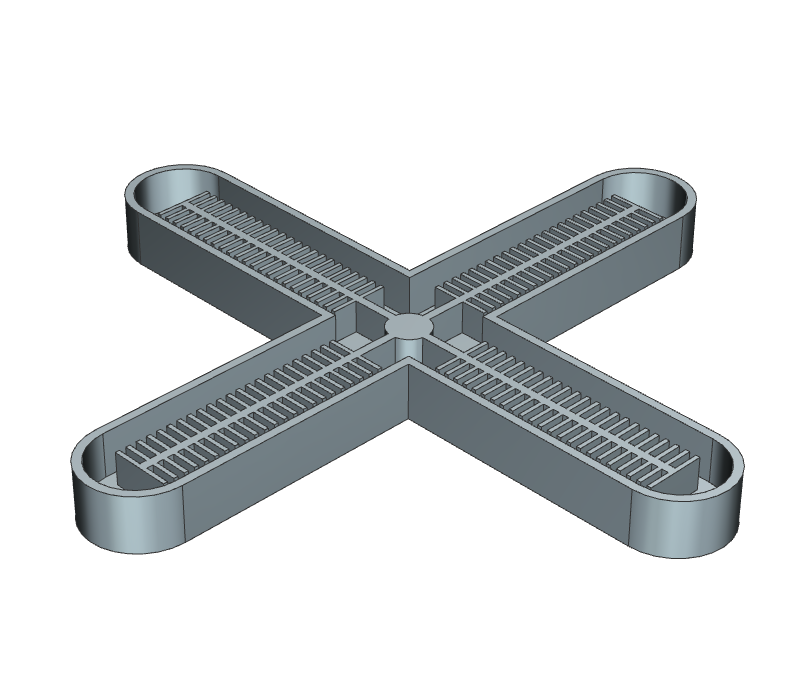
\includegraphics[width=0.9\linewidth]{pics/silikon-gussform.png}
        \caption{Die Gussform (CAD-Modell)}
        \label{fig:silikon-gussform}
    \end{subfigure}
    \begin{subfigure}{0.5\textwidth}
        \centering
        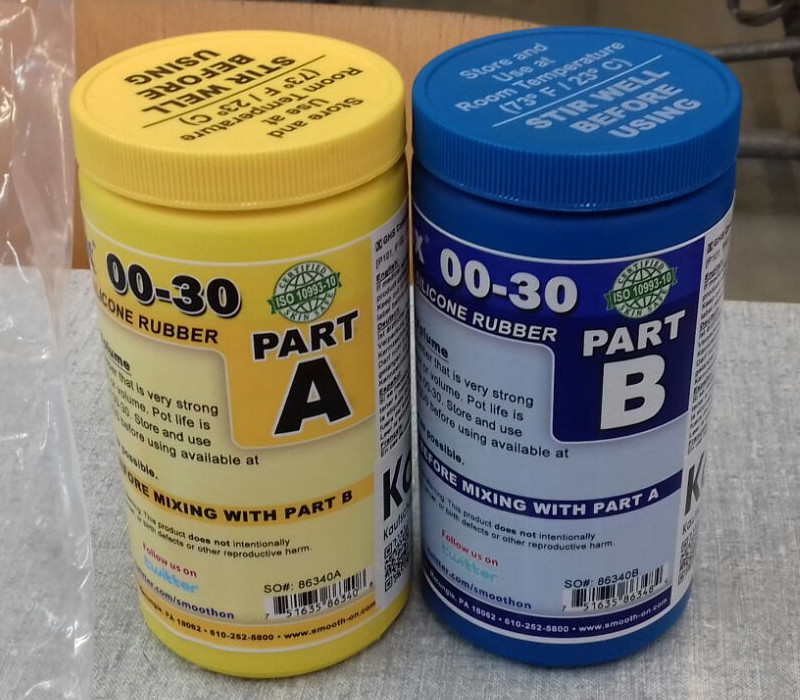
\includegraphics[width=0.9\linewidth]{pics/silikon-komponenten.jpg}
        \caption{Die beiden Silikon-Komponenten}
        \label{fig:silikon-komponenten}
    \end{subfigure}
    \vskip\baselineskip
    \begin{subfigure}{0.5\textwidth}
        \centering
        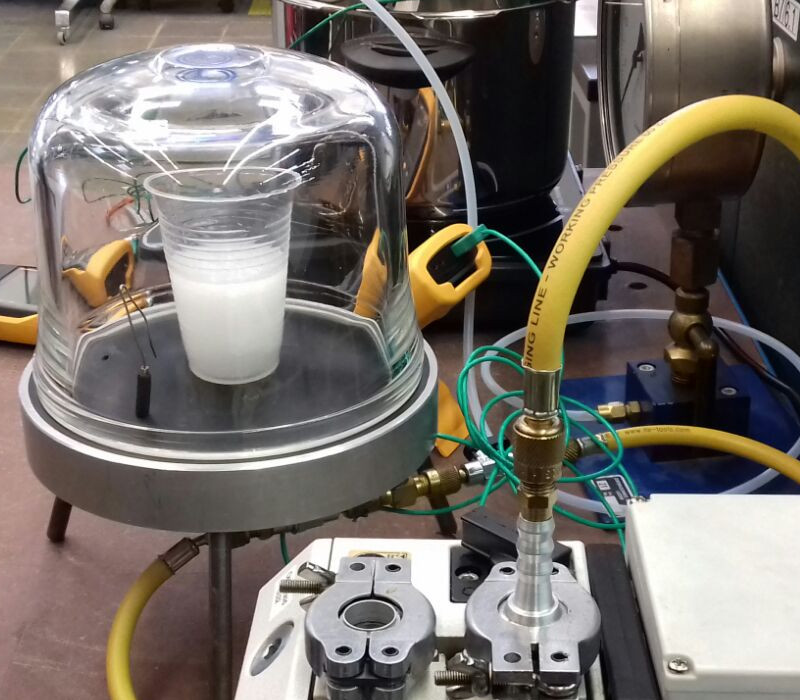
\includegraphics[width=0.9\linewidth]{pics/silikon-vakuum.jpg}
        \caption{Die Silikonmischung unter der Vakuumglocke}
        \label{fig:silikon-vakuum}
    \end{subfigure}
    \begin{subfigure}{0.5\textwidth}
        \centering
        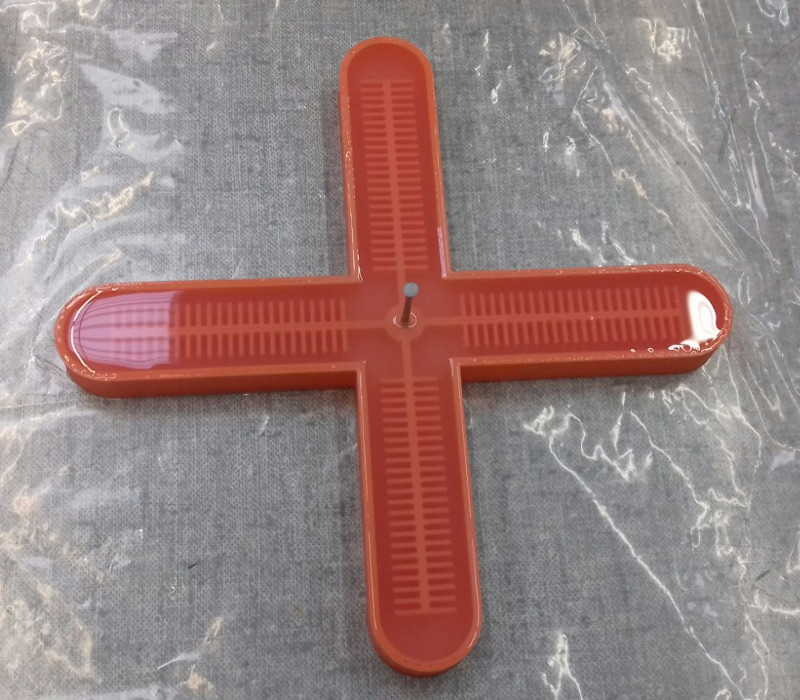
\includegraphics[width=0.9\linewidth]{pics/silikon-giessen.jpg}
        \caption{Das Giessen des Silikongreifers}
        \label{fig:silikon-giessen}
    \end{subfigure}
    \label{fig:herstellung-silikongreifer}
    \caption{Die Herstellung des Silikongreifers}
\end{figure}

\begin{enumerate}
\item In einem ersten Schritt wurde die eigentliche Gussform in CAD geplant und anschliessend 3D gedruckt (\imgref{fig:silikon-gussform}).
\item Anschliessend wurden je $30g$ von den zwei Silikonkomponenten in einem Plastikbecher zusammengeführt und rund drei Minuten lang vermischt (\imgref{fig:silikon-komponenten}). Dabei entstanden kleine Luftblasen, welche unbedingt entfernt werden mussten, da sie allenfalls den eigentlichen Greifarm hätten schwächen können und dadurch keine vollständige Dehnung des Greifers gewährleistet gewesen wäre.
\item Um die Luftblasen zu entfernen, wurde das Silikongemisch unter eine Vakuumglocke gestellt (\imgref{fig:silikon-vakuum}). Die Bläschen wurden dabei aus dem Silikon gesogen. Sobald alle Bläschen beseitigt waren, wurde das Gemisch in die zuvor angefertigte Form gegossen (\imgref{fig:silikon-giessen}). Diese wurde bei Zimmertemperatur insgesamt vier Stunden stehen gelassen, sodass sich das Silikongemisch verfestigen konnte.
\item Weitere $30g$ desselben Silikongemischs wurden in einer dünnen Schicht auf ein Stück Stoff gegossen. Das bereits feste Silikonteil wurde auf die noch flüssige Silikonschicht platziert. Dadurch wurde die Greifhand rückseitig verschlossen. Der Zweck des Stoffes bestand darin, die gewünschte Greifbewegung zu ermöglichen. Durch den Stoff wird verhindert, dass sich die untere Seite des Greifarms ausdehnen kann. Somit verformt sich nur die obere Seite des Greifers, wodurch die gewünschte Greiffingerkrümmung gewährleistet wird und die gegebene Last gefasst werden kann. 
\item Um die bereits oben genannte Luftzufuhr zu ermöglichen, wurde ein zuvor ebenfalls aus Silikon angefertigter Zylinder mit einem Luftkanal an der oberen Seite der Greifhand befestigt. Erstaunlicherweise konnten alle Silikonteile, ob nun bereits in verfestigtem oder noch flüssigem Zustand, mit Silikonresten nahtlos verbunden werden.
\item Die vollständige Greifhand wurde nach vier Stunden in einem abschliessenden Schritt für rund zwei Stunden bei $80\degree C$ in einem Industrieofen erwärmt, um eine maximale Dehnung und Festigkeit zu gewährleisten. Dies wurde vom Silikonhersteller empfohlen \shortcite[Curing/Post Curing]{silikon}.
\end{enumerate}

\subsubsection{Belastungstest}

Der Silikongreifer wurde darauf getestet, ob im aufgeblasenen Zustand die Dehnung und Festigkeit ausreicht. Für das gewünschte Volumen musste 5 mal gepumpt werden, der Riss erfolgt erst bei 30 Mal pumpen. Dies zeigte, dass die fünf notwendigen Pumpvorgänge weit entfernt vom kritischen Volumen sind und die Festigkeit und Dehnung den Anforderungen mehr als gerecht werden. Da einige Rippen im inneren ausgerissen sind, wurde die Gussform angepasst. Die Anzahl Rippen wurde verringert, dafür sind sie in der neueren Form breiter. Ob genug Reibung zwischen Greifer und Last ist, konnte direkt an der Last getestet werden, indem der Greifer aufgeblasen und übertrieben starken Schwingungen ausgesetzt wurde.

\subsection{Ultraschallsensor}
\label{sec:versuch-ultraschallsensor}

Um die Messgenauigkeit des Ultraschallsensors zu Testen, wird der HC-SR04 an den Raspi angeschlossen und über ein Python-Skript in Betrieb genommen. Die gemessenen Distanzen werden direkt auf der Konsole ausgegeben. Getestet wird direkt auf dem Parcours. Der Sensor ist auf einem Steckbrett angebracht und auf den Masten am Ende des Seils gerichtet.
Es werden immer 14 Messungen durchgeführt und aufgelistet. Zuerst wird die gesamte Länge ($337cm$) gemessen. Danach ab $200cm$ in jeweils in Schritten von $20cm$ bis zu $10cm$. Nun werden noch Messungen bei $5cm$, $2.5cm$, und $1.5cm$ durchgeführt. Von allen Messgruppen wird jeweils der Durchschnitt (Mean) und Median bestimmt. 

\begin{figure}[]
    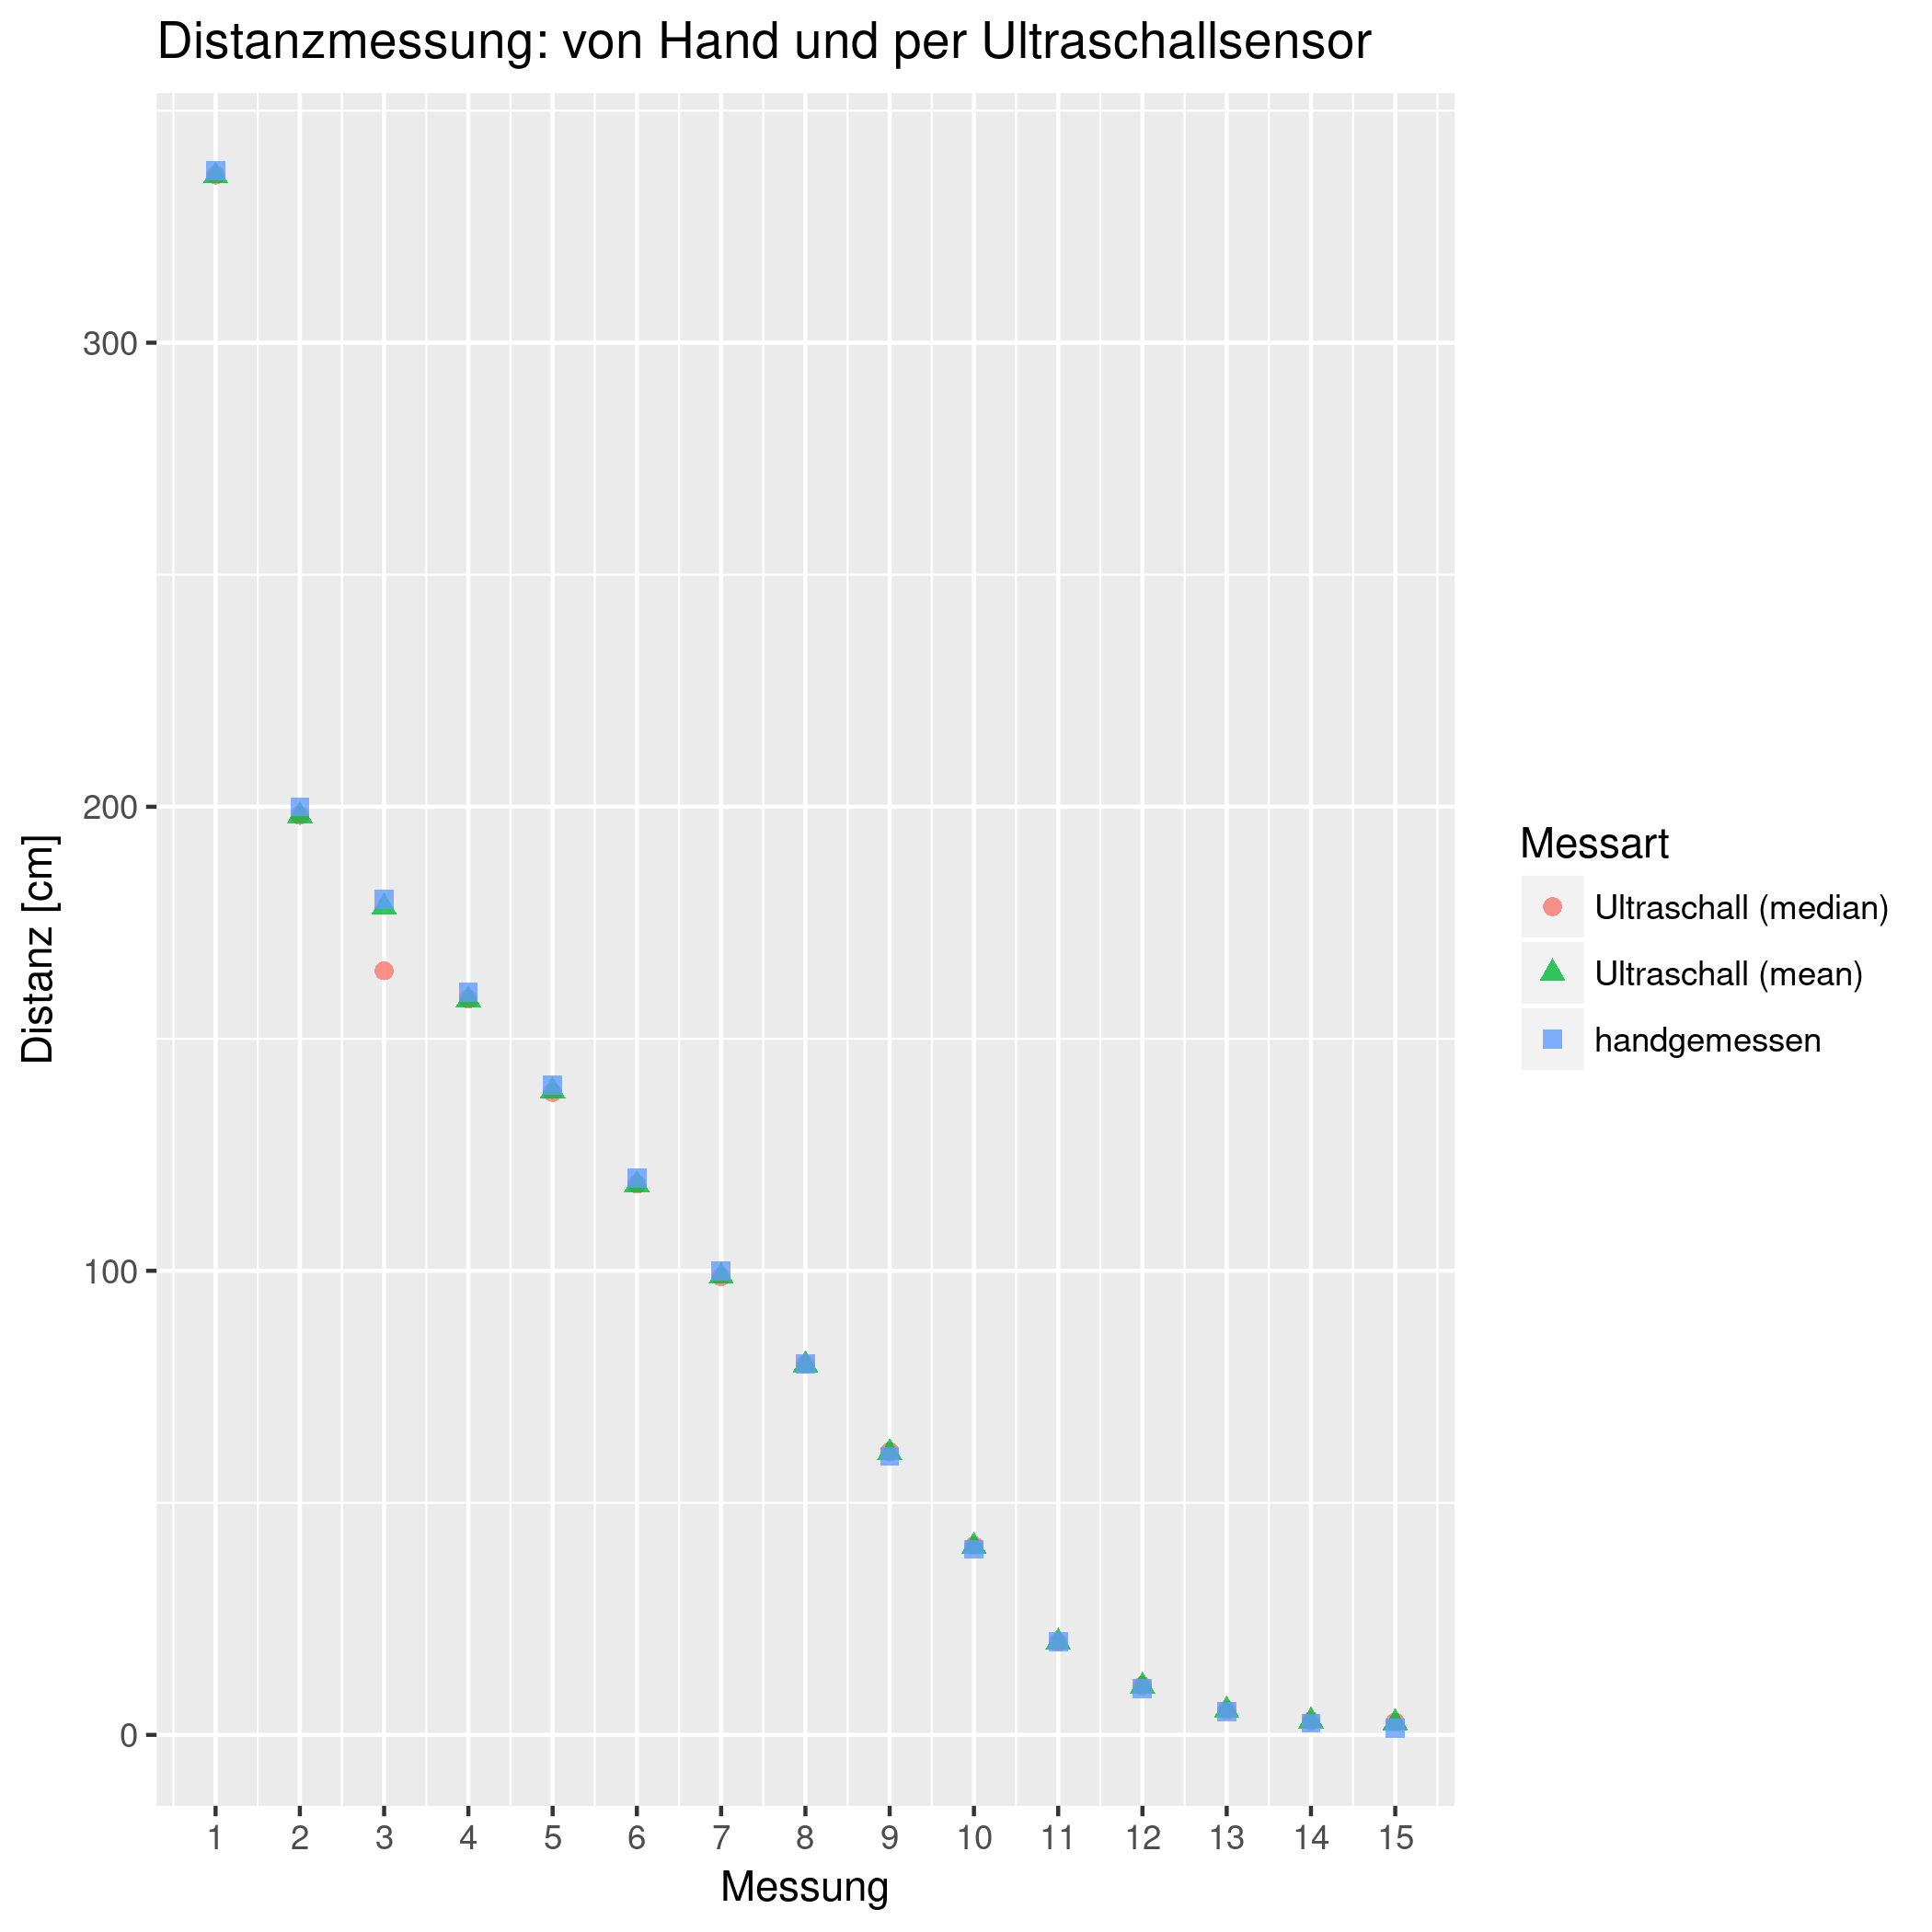
\includegraphics[width=\linewidth]{graphs/ultraschall.png}
    \caption{Die Messungen mit dem Ultraschallsensor}
    \label{fig:graph-ultraschallsensor}
\end{figure}

Zwischendurch kann es zu Messungen kommen, die komplett falsch sind. So z.B bei $180cm$, als ein Wert von $59.1cm$ gemessen wurde. Diese sind aber extrem selten. Um dem entgegenzuwirken, kann der Median der Messgruppe verwendet werden. Anders als beim Mittelwert (Mean) bewirkt ein solcher «Ausreisser» keine Änderung des Endresultates. Der Median ist also wesentlich robuster als der Mittelwert. Ab einer Distanz von $100cm$ misst der Ultraschallsensor tendenziell eher zu wenig: ca. $2cm$ fehlen meist. Unter $100cm$ sind die gemessenen Distanzen erstaunlich genau. Der Fehler des Medians beträgt nie mehr als 2.5\%. Schön zu sehen ist auch die minimale Messdistanz des Sensors bei ca. $3cm$. Unterhalb dieser Grenze können keine genauen Messdaten mehr geliefert werden. Dies stellt aber kein Problem dar, da der Ultraschallsensor einfach so am Gerät platziert wird, dass dieser nie unter dieser Messgrenze messen muss.

\imgrefplain{fig:graph-ultraschallsensor} veranschaulicht die Messungen. Pro Messpunkt werden drei Werte einander gegenübergestellt: die handgemessene Distanz, der Median der Ultraschallmessung und der Mittelwert der Ultraschallmessung. Die drei Punkte liegen dermassen nahe beieinander, dass von blossem Auge kaum Abweichungen auszumachen sind. Einzig bei der dritten Messung ist beim Mittelwert eine grosse Abweichungen zu sehen. Das liegt daran, dass der Sensor teilweise fehlerhafte Daten liefert, und dass der Mittelwert sehr anfällig für «Ausreisser» ist. Aus diesem Grund soll sich die Steuerung auf den Median verlassen.

\subsection{Elektromagnet}
\label{app:elektromagnet}

Als Alternative zum Silikongreifer wurde ein Elektromagnet getestet. Als Modell wurde der Intertec ITS-PE3529-24VD \shortcite{elektromagnet} verwendet. Dieser Elektromagnet kann bis zu $300N$ anheben. Für das Abladen werden $24V$ und $1.16A$ benötigt. Die Speisung wird jedoch nur für das Abladen der Last benötigt. Solange man den Magneten nicht speist, wird die Last voll angezogen. Für den Versuch wurde eine Last verwendet, welche etwas mehr als $2.6kg$ wiegt (\imgref{fig:waage}).

\begin{figure}[]
    \centering
    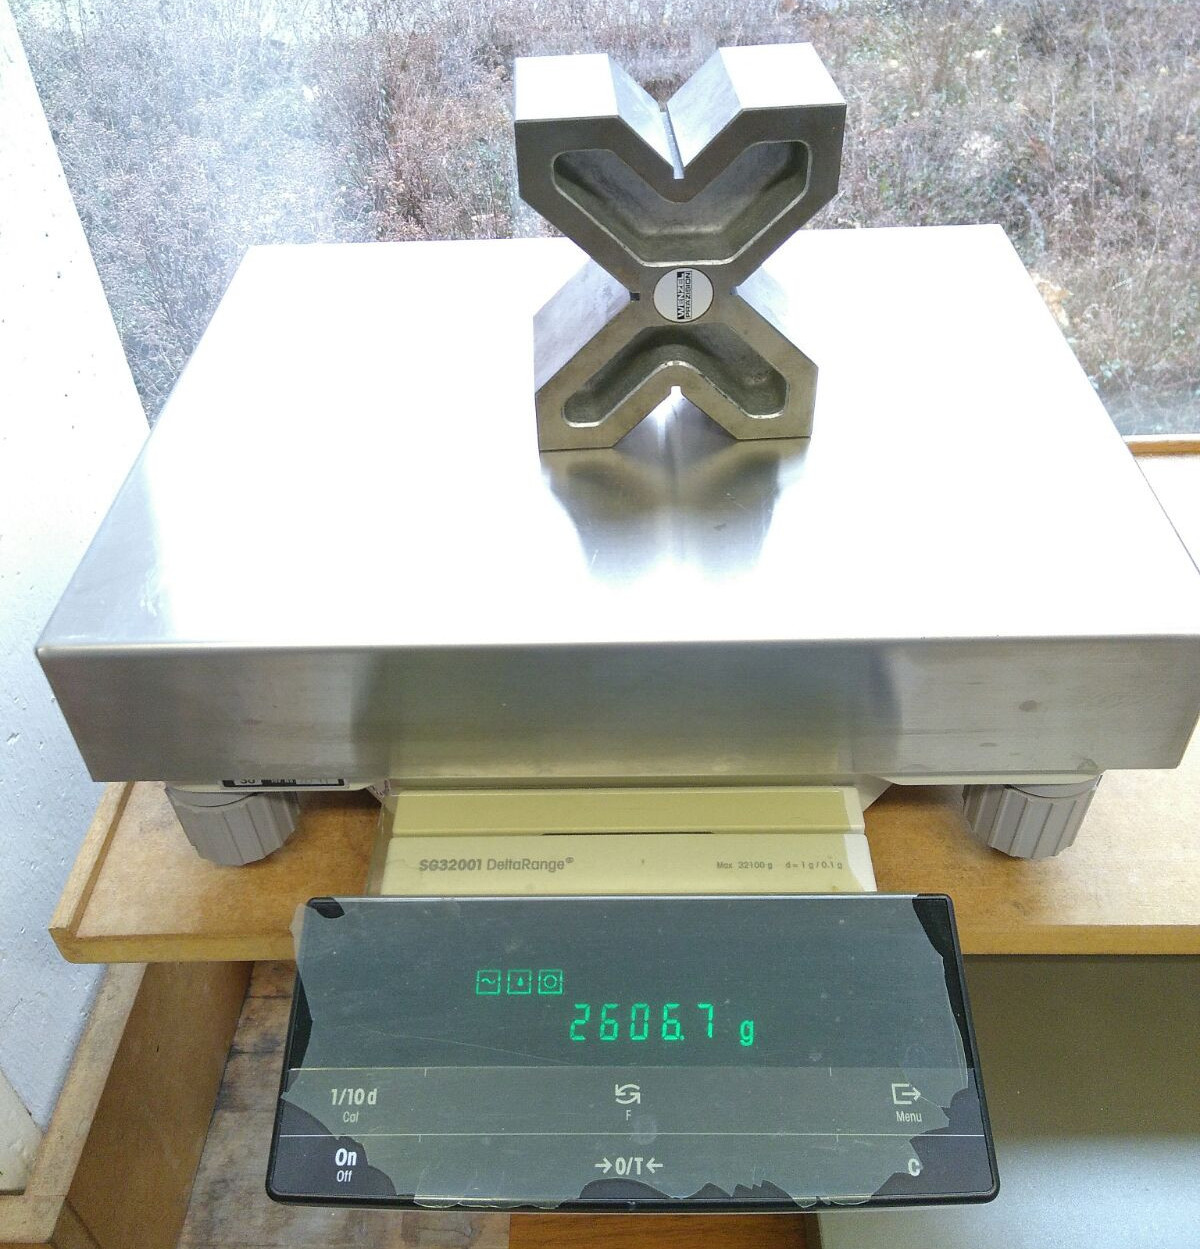
\includegraphics[width=0.5\linewidth]{pics/waage.jpg}
    \caption{Das Gewicht der Last, die mit dem Elektromagneten angehoben wurde}
    \label{fig:waage}
\end{figure}

Die Last von $2.6kg$ konnte ohne Probleme angehoben werden, wie \imgrefplain{fig:anheben} zeigt.

\begin{figure}[]
    \centering
    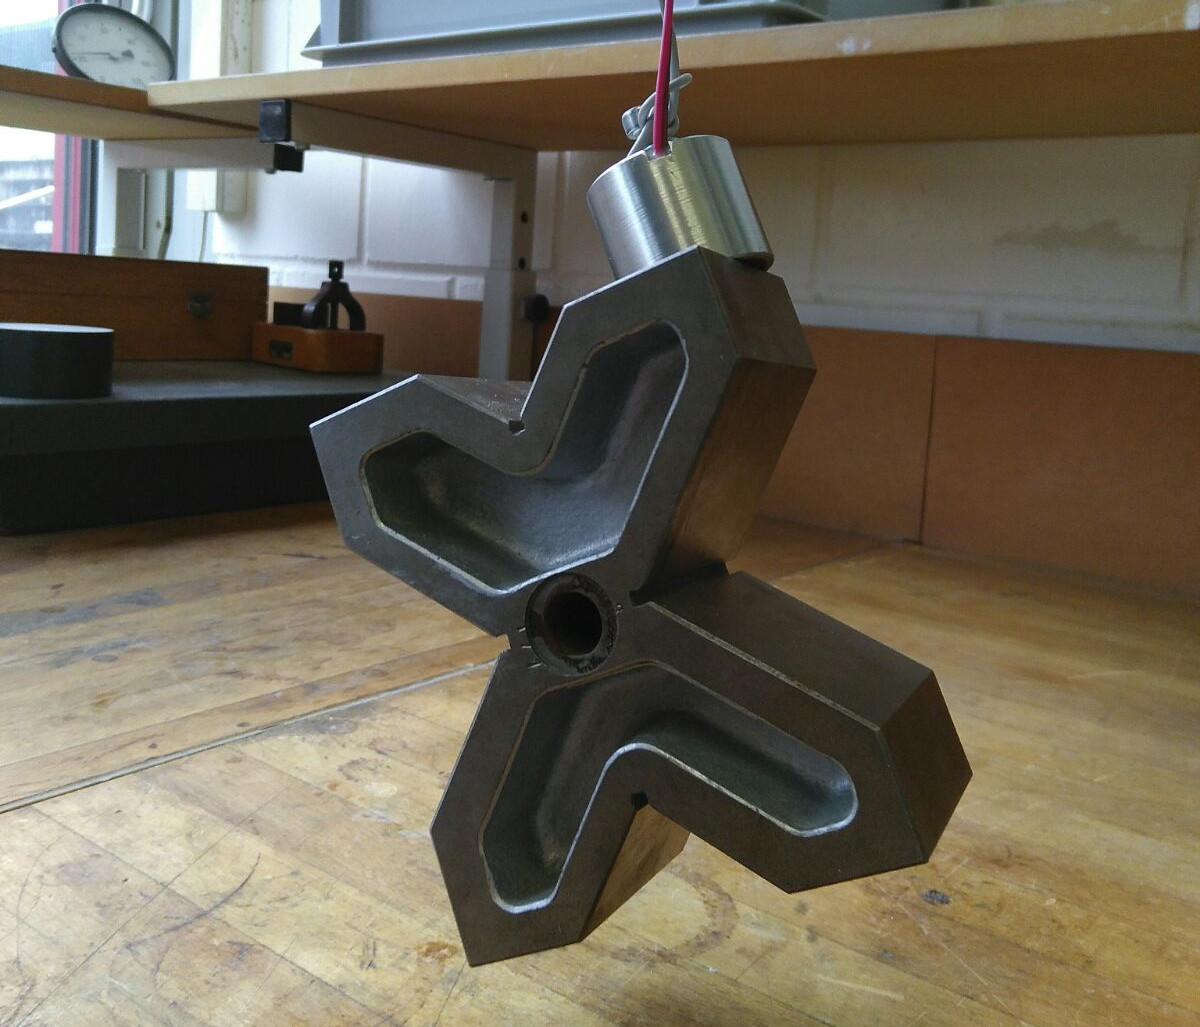
\includegraphics[width=0.5\linewidth]{pics/anheben.jpg}
    \caption{Die vom Elektromagneten angehobene Last}
    \label{fig:anheben}
\end{figure}

\section{Meilensteinberichte}

Die Meilensteinberichte werden als separates Dokument (\texttt{Anhang-G\_\hyp{Meilen\-stein\-berichte.pdf}}) abgegeben.

\section{Protokolle}

Die Protokolle werden als separates Dokument (\texttt{Anhang-H\_Protokolle.pdf}) abgegeben. Sie beinhalten eine wöchentliche Übersicht über die Tätigkeiten aller Gruppenmitglieder.

\section{Gruppenziele}
\label{app:gruppenziele}

\begin{enumerate}[leftmargin=*]
\setlength\itemsep{0.2em}
\item Wir wollen gut zusammen arbeiten ‒ auch über die Fachbereiche hinweg.
\item Wir wollen Spass an der Arbeit haben.
\item Wir wollen etwas lernen ‒ in unserem Fachbereich und fachbereichübergreifend.
\item Wir wollen, dass jedes Gruppenmitglied seinen Beitrag leistet.
\item Wir wollen eine sichere, zuverlässige und für alle verständliche Lösung erarbeiten, nicht den Wettbewerb um jeden Preis gewinnen.
\end{enumerate}

\section{Projektplan}
\label{app:projektplan}

Der Projektplan wird als separates Dokument (\texttt{Anhang-J\_Projektplan.pdf}) abgegeben.
